%  main.tex -- AHPCAI 2026 short paper (SPIE proceedings class)
%  Build: pdflatex main && bibtex main && pdflatex main && pdflatex main
%  Length target: 6 pages (conference limit; page 7 onwards costs extra).
%
%  NUMBER PROVENANCE: every figure in this paper was produced by the
%  harness in the public repository (harness/link_measure.py,
%  record_breakdown.py, session_ticket_probe.py) against OpenSSL 3.5.7,
%  and is stored under results/.  None of it is modelled.

\documentclass[]{spie}  % US letter paper

\usepackage{graphicx}
\usepackage{booktabs}
\usepackage{url}

\title{Five ways to mismeasure a post-quantum TLS 1.3 handshake
on a narrowband link}

\author{Xiaoyu Huang\supit{ab,*} \quad Yiliang Han\supit{ab} \quad
Shuaishuai Zhu\supit{ab} \quad Hui Wu\supit{ab} \quad
Zhongqiang Liu\supit{ab}
\skiplinehalf
\supit{a}Engineering University of PAP, Xi'an, 710086, Shaanxi, China; \\
\supit{b}Key Lab of the Armed Police Force for Network and Information
Security, Xi'an, 710086, Shaanxi, China
}

\authorinfo{Send correspondence to Xiaoyu Huang.\\
X.~Huang: E-mail: 19591587786@163.com}

\begin{document}
\maketitle

\begin{abstract}
Post-quantum migration is increasingly argued from measurements: run the
new primitives on a real stack and report what the handshake costs. On a
narrowband command-and-control link such numbers are hard to win and easy
to lose, because the failure modes of the measurement itself produce
values that look exactly like results. We document five ways our own
first pass was wrong, each of which produced a plausible number: a token
bucket that credited the same wait twice and made the link run 53\,\%
fast; an initial burst that gave the first 1.17\,s away free; a server
status page that contributed 72\,\% of what was being counted; session
tickets that fell inside the measurement window on some runs and outside
it on others, moving the byte count by 12\,\%; and a certificate-authority
option that copied a 5.7-kB certificate into every session ticket,
inflating the reported handshake by 54.7\,\%. Each pitfall is stated with
its symptom, its magnitude, and the check that caught it. The checks
compose into a protocol --- record-layer attribution, a byte-exact
cross-check against the standards, per-direction totals, and a canonical
flag set --- that we recommend to anyone measuring TLS on a constrained
link. Applied to a mutual-authentication ML-KEM-768$+$ML-DSA-65 handshake
the protocol yields 20{,}840 bytes, of which 87.9\,\% is identity
material: a number that survives all five checks.
\end{abstract}

\keywords{post-quantum cryptography, TLS 1.3, performance measurement,
constrained links, unmanned aerial vehicles, measurement pitfalls}

\section{INTRODUCTION}
\label{sec:intro}

Post-quantum cryptography has moved from standards to deployment:
FIPS~203 and FIPS~204 specify ML-KEM and ML-DSA\cite{fips203,fips204},
FIPS~205 adds SLH-DSA\cite{fips205}, X.509 identifiers exist for
both\cite{rfc9881,rfc9909}, and mainstream libraries ship
implementations\cite{openssl35}. The migration is forced by Shor's
algorithm\cite{shor1997} and by the harvest-now-decrypt-later argument
that Mosca's inequality quantifies\cite{mosca2018}; the process behind
the standards is documented in\cite{nistir8105} and surveyed
in\cite{bernstein2017,pqcryptoBook}. A growing literature measures what
the primitives cost on the platforms that will have to run them, from
Cortex-M4 cycle counts\cite{pqm4,botros2019} to TLS handshake timings on
desktop stacks\cite{paquin2020,sikeridis2020ndss}, and the first UAV
studies are appearing\cite{xia2024ligkyx,hussien2026pqmavlink}.

Measured numbers in this area travel far. A byte count that enters a
comparison table is quoted, re-quoted, and eventually becomes the basis
of a migration decision, yet the measurement itself is rarely
scrutinised. The errors a measurement harness makes are not random; they
are \emph{plausible}. A status page is traffic on the socket, a session
ticket is part of the handshake, an initial burst is what sockets do ---
each produced a credible number in our own first pass, and nothing about
the number revealed the error.

This paper is an account of five such failures, in the order we met
them, with the magnitude of each and the check that caught it. The
setting is a measurement that was easy to get wrong in several
independent ways at once: a mutual-authentication TLS~1.3 handshake
carrying ML-KEM-768 and ML-DSA-65\cite{fips203,fips204}, measured over
an emulated 9.6-kbps, 250-ms beyond-line-of-sight command-and-control
link of the kind surveyed in\cite{zeng2016} and specified
in\cite{do362}, carrying \mav{} telemetry\cite{mavlink}, where the
whole handshake takes eleven seconds and every artefact is worth
seconds. The contributions are the failure catalogue
(Section~\ref{sec:pitfalls}), a detection protocol assembled from the
checks that caught them (Section~\ref{sec:protocol}), and the corrected
number that survives the protocol (Section~\ref{sec:case}). A fuller
account of the underlying study --- rate, delay and loss sweeps, and a
comparison of remediation options --- is in preparation; this paper
deliberately reports only what is needed to make the measurement
methodology checkable. The harness and all raw measurements are
public\cite{measurepackage}.

\section{TESTBED AND MEASUREMENT CONVENTION}
\label{sec:testbed}

\subsection{Stack and configuration}

All measurements use OpenSSL 3.5.7\cite{openssl35} with TLS~1.3 as
specified in RFC~8446\cite{rfc8446}. The measured configuration is a
mutual-authentication handshake in which both peers present an
ML-DSA-65 certificate\cite{fips204} and the key exchange is the pure
ML-KEM-768 group\cite{fips203}. The other standardised signature family,
SLH-DSA, is not measured here: its smallest parameter set carries
7{,}856-byte signatures\cite{fips205}, which a 9.6-kbps link cannot
absorb in any useful number of handshakes. Research libraries such as
liboqs offer a wider algorithm set but no record layer\cite{liboqs}, and
the record layer is what this paper measures. A classical comparison
configuration
uses X25519 with ECDSA-P256; it measures 1{,}915 bytes and 1.99\,s
against the post-quantum 20{,}840 bytes and 11.27\,s, a factor of
5.66 in time on the link used throughout. Certificates are self-signed
at chain depth one, and session tickets are disabled on both sides by
default --- for a reason that turns out to be pitfall~5.

\subsection{Link emulation}

The client and server run on one host and communicate through a
userspace TCP proxy that applies a token bucket and a fixed one-way
propagation delay per forwarded chunk in each direction: 9.6\,kbps per
direction and 250\,ms, the parameters of a narrowband
beyond-line-of-sight radio. DTLS~1.3 is the transport such a link would
use in practice, but this stack implements DTLS~1.2 only\cite{rfc9147,rfc6347},
whose cipher-suite names encode the authentication algorithm and which
has no ML-KEM group; TLS over TCP is therefore what can be measured,
and the framing difference is a bound rather than a measurement. The throttle was validated against a known
transfer: pushing 12{,}000 bytes through the 9.6-kbps setting yields
9.57\,kbps, within 0.3\,\% of target. Two earlier versions of the
throttle were wrong in ways that were invisible in the handshake numbers
themselves; both are pitfalls~1 and~2 below.

\subsection{Byte accounting convention}

Bytes are counted by a record-layer parser inside the proxy, not by a
socket counter: it records every TLS record with its type and length and
attributes the two plaintext hellos to message types, so everything after
the ServerHello is accounted by record. The client's one-byte liveness
probe occupies a 23-byte record, which every total here includes; the
convention is stated so it can be undone by hand. Byte counts include
5-byte TLS record headers, key-exchange payloads do not.

\section{FIVE PITFALLS}
\label{sec:pitfalls}

Table~\ref{tab:pitfalls} summarises the five failure modes. None of them
is exotic, and that is the point: each produced a number we were ready
to report.

\begin{table}[h]
\caption{The five measurement pitfalls. The middle columns give the
effect each had on the reported number before it was found, and the last
column the change that removed it. No number in this paper predates the
fixes.}
\label{tab:pitfalls}
\begin{center}
\begin{tabular}{@{}p{0.04\textwidth}p{0.27\textwidth}p{0.26\textwidth}p{0.22\textwidth}@{}}
\toprule
\# & Failure mode & Effect on the number & Correction \\
\midrule
1 & Token bucket credited the same wait twice & link ran at 14.73
instead of 9.60\,kbps, 53\,\% fast & allow the balance to go negative \\
2 & Free initial burst of 1{,}400 bytes & 1.17\,s uncharged at
9.6\,kbps & burst set to zero \\
3 & \texttt{-www} status page counted as handshake & about 5\,kB of HTML
against a 1.9\,kB handshake, 72\,\% of the count & server run without
\texttt{-www} \\
4 & \texttt{NewSessionTicket} inside or outside the window & 12\,\% byte
variation between runs & tickets disabled on both sides \\
5 & \texttt{-CAfile} certificate copied into each ticket & 20{,}840
$\to$ 32{,}236 bytes, $+$54.7\,\% & \texttt{-no\_ticket} on the server
as well \\
\bottomrule
\end{tabular}
\end{center}
\end{table}

\textbf{(1) The token bucket credited the same wait twice.} The first
throttle clamped the token balance to zero when a chunk exceeded the
available credit, then refilled from elapsed time on the next call. The
wait already served therefore re-entered the balance as fresh capacity,
and the emulated link ran at 14.73\,kbps against a 9.6-kbps target ---
53\,\% fast. Every completion time in that version of the harness was
compressed, and nothing about the compressed times looked wrong: they
were smooth, monotone in bytes, and stable across runs. The fix is to
let the balance go negative, so that the bucket owes capacity rather
than forgetting the debt.

\textbf{(2) The token bucket handed out a free burst.} With a 1{,}400-byte
initial burst, a short transfer received its first 1{,}400 bytes at no
cost. At 9.6\,kbps that is 1.17\,s of airtime given away, which is not
negligible when the measured handshake takes 11.27\,s: a systematic
10\,\% discount on every transfer, paid to the first 1{,}400 bytes. The
effect is not an artefact of our emulator alone: TCP opens a connection
with a ten-segment initial window\cite{rfc6928}, so a real link hands out
a burst of its own, and the choice here is to remove it and measure
serialisation rather than to leave it unaccounted. The burst is now
zero, which makes serialisation exact. The general lesson is that
throttles must be validated against a known transfer, not trusted to be
conservative.

\textbf{(3) The server's status page was counted as handshake.} An early
version drove \texttt{s\_server} with \texttt{-www}, whose HTML status
page is about 5\,kB and was counted in the byte total. On the classical
configuration this was more than half the reported figure: about 5\,kB
against a 1.9-kB handshake, 72\,\% of what was being counted. The error
survived a plausibility check that should have killed it --- 7\,kB felt
large for a handshake --- because the post-quantum configurations in the
same batch were larger still. The server now runs without
\texttt{-www}.

\textbf{(4) Session tickets fell inside or outside the window.}
\texttt{NewSessionTicket} arrives after the handshake completes, so
whether it fell inside the measurement window depended on link speed and
scheduling. The same configuration varied by 12\,\% in byte count
between runs. This is the failure mode that record-level accounting is
for: a total counter cannot distinguish a handshake that carries tickets
from one that does not, and a window is a policy decision that must be
stated. Tickets are now disabled on both sides, which makes every run
byte-identical.

\textbf{(5) The certificate-authority certificate was embedded in every
ticket.} This is the one that mattered most, because it inflated the
result we most wanted to be true. With client authentication enabled,
\texttt{s\_server} uses its \texttt{-CAfile} both to validate the client
certificate and to build the chain it sends, and with tickets enabled the
CA certificate reappeared inside each \texttt{NewSessionTicket}: the two
post-handshake records grew from 79 bytes each --- what a ticket should
cost --- to 5{,}775 bytes each, 5{,}696 bytes larger, the size of the
certificate plus ticket framing. The server-to-client direction grew
from 10{,}468 to 21{,}860 bytes, and the handshake total from 20{,}840
to 32{,}236 bytes, an inflation of 54.7\,\% (Figure~\ref{fig:artefact}).
Client-side \texttt{-no\_ticket} does not suppress it, because the
ticket is emitted by the server after the handshake; the server must be
given the flag as well. Two details make the account checkable to the
byte. The client's flight gains four bytes at the same time, because
with tickets enabled the client offers the empty \texttt{session\_ticket}
extension, which \texttt{-no\_ticket} suppresses, growing its
\texttt{ClientHello} from 1{,}357 to 1{,}361 bytes; the two directions
therefore grow by 11{,}392 and 4 bytes, and the 11{,}396-byte growth of
the total is their sum. And a 32-kB handshake is not obviously wrong
--- published post-quantum figures are in that range --- so what caught
this was not intuition but attribution: the 5{,}775-byte records were not
explicable from any field of the handshake, and a record that cannot be
attributed has to be investigated rather than averaged in.

\begin{figure}[h]
\begin{center}
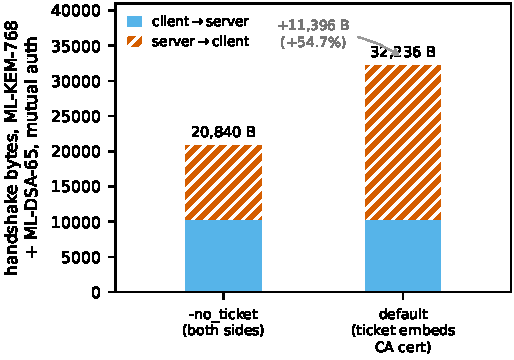
\includegraphics[width=0.62\textwidth]{fig-artefact}
\end{center}
\caption{Pitfall 5. Both bars are the same mutual-authentication
ML-KEM-768$+$ML-DSA-65 handshake. In the left bar the server was started
with \texttt{-no\_ticket} and the two post-handshake records are 79 bytes
each; in the right bar that flag was omitted and the \texttt{-CAfile}
certificate is embedded in each ticket. Reporting the right-hand bar as
the cost of post-quantum authentication would have overstated it by
54.7\,\%.}
\label{fig:artefact}
\end{figure}

\section{A DETECTION PROTOCOL}
\label{sec:protocol}

Five one-off catches are an anecdote; the useful output is the check set
that caught them, which generalises beyond this testbed. We recommend
four checks for any TLS measurement on a constrained link.

\textbf{Attribute by record, not by socket.} Count bytes at the record
layer with a parser that names every record, not with a counter on the
socket or the process. Pitfalls 3, 4 and 5 were all invisible to a total
counter and trivial to a parser: a status page is application data, a
ticket is a named post-handshake record, and an oversized ticket is a
record whose length no handshake field explains. The parser needs no
decryption --- TLS~1.3 record boundaries and lengths are visible without
keys, and the two hellos are plaintext.

\textbf{Cross-check one record against the standards to the byte.} At
least one measured record should be reconstructed from first principles.
The 5{,}549-byte \texttt{Certificate} record is 35 bytes of TLS framing
(5 record header, 16 AEAD tag, 4 handshake header, 1 content type, 1
context length, 3 list length, 3 certificate length, 2 extensions
length) plus 5{,}514 bytes of DER, which is in turn 1{,}952 of ML-DSA-65
public key, 3{,}309 of signature and 253 of X.509
framing\cite{fips204,rfc9881}. Table~\ref{tab:messages} gives the full
per-message reconstruction. A check of this kind is worth more than
repetition: repetition bounds noise, while a byte-exact reconstruction
detects systematic error, and it was exactly this check --- not a
statistic --- that exposed pitfalls 3 and 5.

\begin{table}[h]
\caption{Per-message reconstruction of the corrected handshake. Bytes in
the second column are read off the wire by the record parser; bytes in
the third column follow from FIPS~203/204 and X.509 framing, so the two
columns check each other. Framing rows hold the records that carry no
handshake content: ChangeCipherSpec, the 23-byte liveness probe
(client), the two tickets (server, 79 bytes each here), and
close\_notify.}
\label{tab:messages}
\begin{center}
\begin{tabular}{@{}lrr@{}}
\toprule
Message & Bytes & Contents \\
\midrule
\multicolumn{3}{l}{\emph{client $\to$ server} (total 10{,}372)} \\
\quad \texttt{ClientHello} & 1{,}357 & key share 1{,}192 \\
\quad \texttt{Certificate} & 5{,}549 & DER 5{,}514 $+$ 35 framing \\
\quad \texttt{CertificateVerify} & 3{,}339 & signature 3{,}309 $+$ 30 \\
\quad \texttt{Finished} & 74 & \\
\quad \emph{framing} & 53 & CCS 6, probe 23, close 24 \\
\midrule
\multicolumn{3}{l}{\emph{server $\to$ client} (total 10{,}468)} \\
\quad \texttt{ServerHello} & 1{,}183 & key share 1{,}096 \\
\quad \texttt{EncryptedExtensions} & 28 & \\
\quad \texttt{CertificateRequest} & 107 & \\
\quad \texttt{Certificate} & 5{,}549 & as above \\
\quad \texttt{CertificateVerify} & 3{,}339 & as above \\
\quad \texttt{Finished} & 74 & \\
\quad \emph{framing} & 188 & CCS 6, tickets 158, close 24 \\
\midrule
Total & 20{,}840 & \\
\bottomrule
\end{tabular}
\end{center}
\end{table}

\textbf{Replay with a canonical flag set.} Tickets are disabled on both
sides, the server runs without \texttt{-www}, the client sends a stated
one-byte probe, and the throttle has no burst. The flag set is part of
the method: half of the pitfalls above are impossible with the right
flags, and a measurement that does not state its flags cannot be
reproduced at the byte level at all, because byte counts are a
deterministic function of the flags.

\textbf{Report per-direction totals.} The two flights of a handshake are
10{,}372 and 10{,}468 bytes, and artefacts do not respect their sum: an
oversized ticket inflates only the server's flight, a status page only
whichever side emits it. A single total hides the very asymmetry that
makes an error visible. The 4-byte \texttt{session\_ticket} extension of
pitfall~5 would have been unfindable in a 32{,}236-byte total; in
per-direction totals it is the only unexplained delta on the client
flight.

Two further practices bound the residual error. The throttle is
validated against a known transfer (within 0.3\,\% here), and the
measurement is repeated: five runs give a standard deviation of 0.011\,s,
or 0.10\,\% of the mean. Repetition carries a caution of its own, though
--- in a batch of fifteen runs two stalled by 0.4--0.5\,s with no
injected loss, and while the means reproduced across batches within
1\,\%, the spreads did not. Repetition measures noise on the day; on a
constrained link the tails are part of the measurement.

\section{CASE STUDY: THE NUMBER THAT SURVIVES}
\label{sec:case}

Applying the protocol to the post-quantum handshake gives 20{,}840 bytes
in 11.27\,s at 9.6\,kbps per direction and 250\,ms one-way. Of those,
2{,}530 bytes (12.1\,\%) are the key exchange --- both hellos and their
record headers --- and 18{,}310 (87.9\,\%) are identity material: two
5{,}549-byte certificates, two 3{,}339-byte \texttt{CertificateVerify}
signatures, and the records that carry them. Each of the five pitfalls
would have changed this headline. Pitfalls 1--3 distort the time axis;
pitfalls 4 and 5 distort the byte axis, and pitfall 5 inflates the
reported handshake by more than half while leaving the true handshake
untouched. The 5.66$\times$ time ratio between the post-quantum and classical
configurations --- the number most likely to be quoted --- becomes a byte
ratio of 16.8$\times$ (32{,}236 against 1{,}915) and a time ratio of
about 8.3$\times$ if the right-hand bar of Figure~\ref{fig:artefact} is
reported by mistake. None of the checks that caught these
errors costs more than a few hundred lines of parsing code and the
discipline to state a flag set; all are reproducible from the public
repository\cite{measurepackage}.

\section{RELATED WORK}
\label{sec:related}

Benchmarking of post-quantum primitives on constrained hardware is well
developed\cite{pqm4,botros2019}, and the cost of the primitives inside
TLS has been measured on desktop
stacks\cite{paquin2020,sikeridis2020ndss,sikeridis2020conext}, while
KEMTLS shows how far the handshake itself can be restructured to remove
the certificate signature\cite{schwabe2020kemtls}.
That literature reports results; what it rarely reports is the failure
modes of the measurement itself, which are exactly what a byte-level
methodology paper can contribute. UAV-specific studies report a single
capture\cite{xia2024ligkyx} or a simulation\cite{hussien2026pqmavlink},
in neither case with a stated accounting convention. Our own record is
no cleaner than the field's, which is the reason for this paper: we
reported at one point that OpenSSL 3.5.7 could not resume a TLS~1.3
session at all, when the correct reading was that this server, in this
configuration, issues no ticket to resume from --- the observation that
falsified the first reading was the absence of a
\texttt{NewSessionTicket} record in the log, not a different statistic.
Every correction in this paper is stated with the observation that
falsified the previous reading.

\section{CONCLUSION}
\label{sec:conclusion}

Measured numbers about post-quantum handshakes are becoming the evidence
base for migration decisions, and the measurement harness is the part of
that evidence base that gets the least scrutiny. We document five
failure modes that each produced a plausible number on a real TLS~1.3
stack, the largest inflating the result by 54.7\,\% and the subtlest
moving it by four bytes, and we compress the checks that caught them
into a four-part protocol: record-layer attribution, a byte-exact
standards cross-check, a canonical flag set, and per-direction totals.
The protocol costs little, needs no decryption, and converts a byte
count from a claim into a derivation. We recommend it --- and the
reporting of negative results like these --- as standard practice for
constrained-link measurement.

\acknowledgments
The measurement harness was developed with the assistance of AI coding
tools under the authors' direction; all results were reviewed and
reproduced by the authors, and the harness and raw measurements are
publicly available.

\bibliography{refs}
\bibliographystyle{spiebib}

\end{document}
